\RequirePackage{luatex85}

\documentclass[tikz]{standalone}

\usepackage[siunitx]{circuitikz}

\usetikzlibrary{calc}

\tikzset{
  neuron/.style={
    % The shape:
    circle,
    % The size:
    minimum size=6mm,
    % The border:
    very thick,
    draw=blue!50!black!50,
        % The filling:
    top color=white,
    bottom color=blue!50!black!20, % and something else at the bottom
    % Font
    font=\itshape,
    % padding around node
    % outer sep=2mm
  }
}

\begin{document}

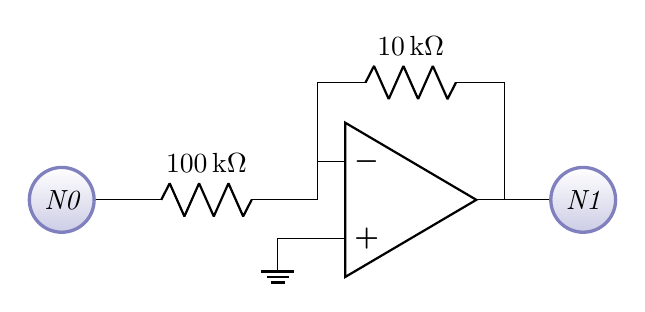
\begin{tikzpicture}

  % \draw (0, 0) node (follower) [op amp] {}
  %       (follower.-) to
  %       ++(0, 1) coordinate (follower end o)
  %       to (follower end o -| follower.out) to (follower.out);

  \node at (0, 0) (n0) [neuron] {N0};

  \node (inverter) [op amp] at ($(n0.east) + (4, 0)$) {};

  \draw (n0.east) to [R, l=100<\kilo\ohm>] (n0.east -| inverter.-) to (inverter.-);

  \draw (inverter.+) to ++(-0.5, 0) node [rotate=0, ground] {};

  \draw (inverter.-) to ++(0, 1) coordinate (inverter end o) to [R, l=10<\kilo\ohm>] (inverter end o -| inverter.out) to (inverter.out) to ++(1, 0) node [neuron] {N1};

\end{tikzpicture}

\end{document}
